\documentclass[a4paper,12pt]{article}
\usepackage[a4paper,top=1.3cm,bottom=2cm,left=1.5cm,right=1.5cm,marginparwidth=0.75cm]{geometry}
\usepackage{setspace}
\usepackage{cmap}
\usepackage{mathtext}
\usepackage[T2A]{fontenc}
\usepackage[utf8]{inputenc}
\usepackage[english,russian]{babel}
\usepackage{multirow}
\usepackage{graphicx}
\usepackage{wrapfig}
\usepackage{tabularx}
\usepackage{float}
\usepackage{longtable}
\usepackage{hyperref}
\hypersetup{colorlinks=true,urlcolor=blue}
\usepackage[rgb]{xcolor}
\usepackage{amsmath,amsfonts,amssymb,amsthm}
\usepackage{icomma}
% $\mathtoolsset{showonlyrefs=false}$
\usepackage{euscript}
\usepackage{mathrsfs}
\usepackage{float}
\usepackage{amsmath}
\setlength{\parindent}{1cm} % Устанавливает отступ в 1.5 см для всех абзацев


\DeclareMathOperator{\sgn}{\mathop{sgn}}
\newcommand*{\hm}[1]{#1\nobreak\discretionary{}
	{\hbox{$\mathsurround=0pt #1$}}{}}

\title{\textbf{Отчёт о выполненой лабораторной работе \\ \textit{Получение и измерение вакуума (2.3.1)}}}

\author{Каплин Артём Б01-402}
\date{5 мая 2025}


\begin{document}

\maketitle
	
	\section{Введение}
	
	\textbf{Цель работы:} 1) измерение объемов форвакуумной и высоковакуумной частей установки; 2) определение скорости откачки системы в стационарном режим, а также по ухудшению и по улучшению вакуума.\\
    \\
    \textbf{Оборудование:} вакуумная установка с манометрами: масляным, термопарным, и ионизационным; источник питания; видеокамера телефона..
	
	\section{Экспериментальная установка}

    \begin{figure}[h]
        \center{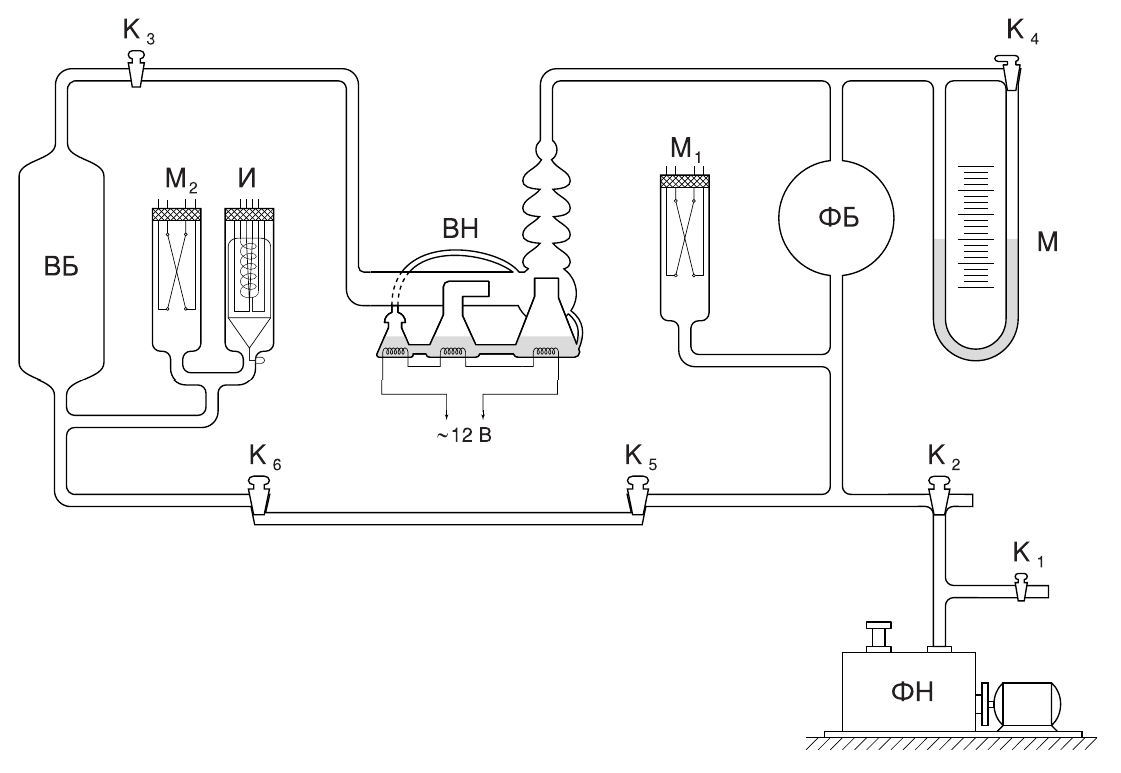
\includegraphics[width=0.8\textwidth]{ustanovka (1).png}}
        \caption{Схема экспериментальной установки.}
        \label{ris:ustanovka}
    \end{figure}

    \paragraph{}
    Установка изготовлена из стекла и состоит из форвакуумного баллона (ФБ), высоковакуумного диффузионного насоса (ВН), высоковакуумного баллона (ВБ), масляного (М) и ионизационного (И) манометров, термопарных манометров ($M_1$ и $M_2$), форвакуумного насоса (ФН) и соединительных кранов (Рис. \ref{ris:ustanovka}).

    \begin{figure}[h]
        \center{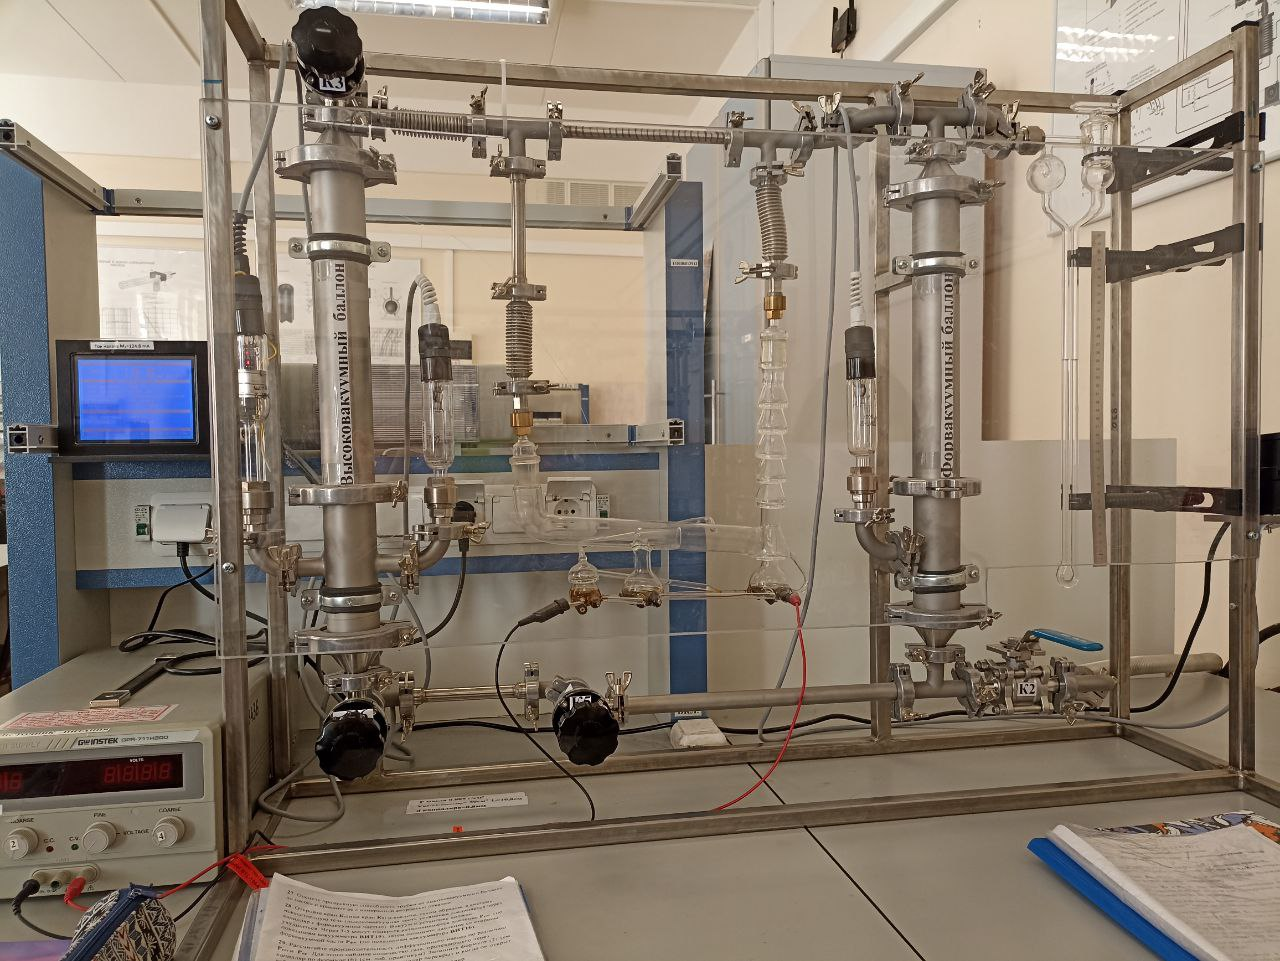
\includegraphics[width=0.7\textwidth]{photo_2025-05-06_00-25-36.jpg}}
    \end{figure}

    \paragraph{Маслянный манометр:}
    Представляет собой U-образную трубку, до половины наполненную вязким маслом, обладающим весьма низким давлением насыщенных паров. Так как плотность масла мала, $\rho = 0,885 \frac{\text{г}}{\text{см}^3}$ , то при помощи манометра можно измерить только небольшие разности давлений (до нескольких торр).

    \paragraph{Термопарный манометр:}
    Чувствительным элементом манометра является термопара, заключенная в стеклянный баллон. Устройство термопары пояснено на (Рис. \ref{ris:termoparni_monometr}). По нити накала НН пропускается ток постоянной величины. Термопара ТТ присоединяется к милливольтметру, показания которого определяются температурой нити накала и зависят от отдачи тепла в окружающее пространство. Потери тепла определяются теплопроводностью нити и термопары, теплопроводностью газа, переносом тепла конвективными потоками газа внутри лампы и теплоизлучением нити (инфракрасное тепловое излучение). В обычном режиме лампы основную роль играет теплопроводность газа. При давлениях >1 торр теплопроводность газа, а вместе с ней и ЭДС термопары практически не зависят от давления газа, и прибор не работает. При улучшении вакуума средний свободный пробег молекул становится сравнимым с диаметром нити, теплоотвод падает и температура спая возрастает. При вакууме $\sim 10^{-3}$ торр теплоотвод, осуществляемый газом, становится сравнимым с другими видами потерь тепла и температура нити становится практически постоянной. Градуировочная кривая термопарного манометра приведена на (Рис. \ref{ris:termopara_graduirovka}).

    \begin{figure}[h]
    \centering
    \begin{minipage}{0.3\textwidth}
        \centering
        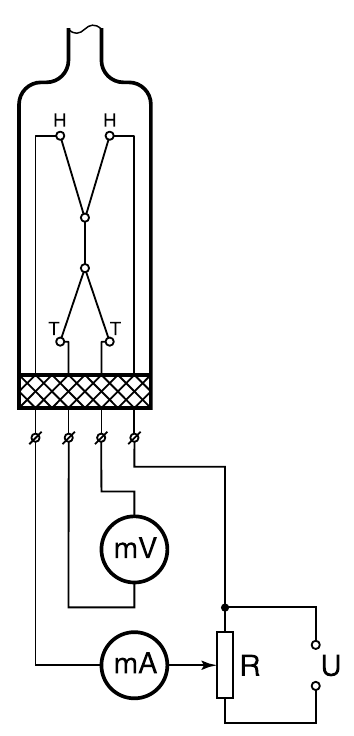
\includegraphics[width=0.7\textwidth]{termoparni_monometr.png}
        \caption{Схема термопарного манометра.}
        \label{ris:termoparni_monometr}
    \end{minipage}\hfill
    \begin{minipage}{0.7\textwidth}
        \centering
        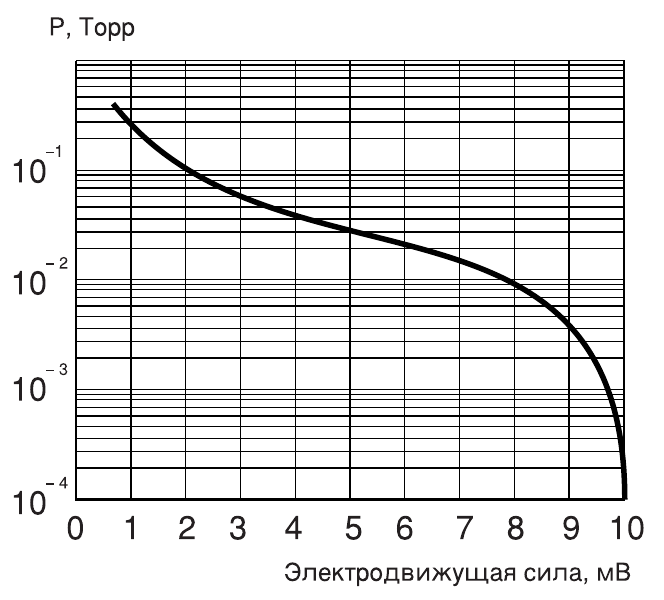
\includegraphics[width=0.7\textwidth]{termopara_graduirovka.png}
        \caption{Градуировочная кривая термопарного манометра.}
        \label{ris:termopara_graduirovka}
    \end{minipage}
    \end{figure}

    \paragraph{Ионизационный манометр:}
    Схема ионизационного манометра изображена на (Рис. \ref{ris:ionizacionni_monometr}). Он представляет собой трехэлектродную лампу. Электроны испускаются накаленным катодом и увлекаются электрическим полем к аноду, имеющему вид спирали. Проскакивая за ее витки,электроны замедляются полем коллектора и возвращаются к катоду, а от него вновь увлекаются к аноду. Прежде чем осесть на аноде, они успевают много раз пересечь пространство между катодом и коллектором. На своем пути электроны ионизуют молекулы газа. Ионы, образовавшиеся между анодом и коллектором, притягиваются полем коллектора и определяют его ток. Ионный ток в цепи коллектора пропорционален плотности газа и поэтому может служить мерой давления. Калибровка манометра верна, если остаточным газом является воздух. Накаленный катод ионизационного манометра перегорает, если давление в системе превышает $10^{-3}$ торр. Поэтому включать ионизационный манометр можно, только убедившись по термопарному манометру, что давление в системе не превышает $10^{-3}$ торр. При измерении нить ионизационного манометра сильно греется. При этом она сама, окружающие ее электроды и стенки стеклянного баллона могут десорбировать поглощенные ранее газы. Выделяющиеся газы изменяют давление в лампе и приводят к неверным показаниям. Поэтому перед измерениями ионизационный манометр прогревается (обезгаживается) в течение 10–15 мин. Для прогрева пропускается ток через спиральный анод лампы.

    \vspace{1cm}

    \begin{figure}[h]
        \center{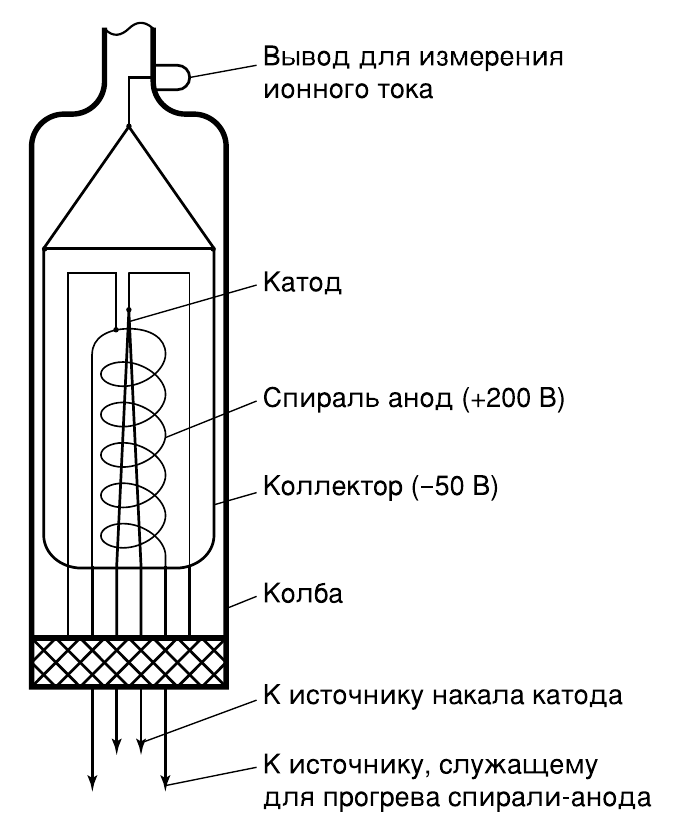
\includegraphics[width=0.3\textwidth]{ionizacionni_monometr.png}}
        \caption{Схема ионизационного манометра.}
        \label{ris:ionizacionni_monometr}
    \end{figure}

    %\newpage

    \paragraph{Диффузионный насос:}
    Откачивающее действие диффузионного насоса основано на диффузии (внедрении) молекул разреженного воздуха в струю паров масла. Попавшие в струю молекулы газа увлекаются ею и уже не возвращаются назад. Устройство одной ступени масляного диффузионного насоса схематически показано на (Рис. \ref{ris:diffuzionni_nasos}) (в лабораторной установке используется несколько откачивающих ступеней). Масло, налитое в сосуд А, подогревается электрической печкой. Пары масла поднимаются по трубе Б и вырываются из сопла В. Струя паров увлекает молекулы газа,которые поступают из откачиваемого сосуда через трубку ВВ. Дальше смесь попадает в вертикальную трубу Г. Здесь масло осаждается на стенках трубы и маслосборников и стекает вниз, а оставшийся газ через трубу ФВ откачивается форвакуумным насосом. Диффузионный насос работает наиболее эффективно при давлении, когда длина свободного пробега молекул воздуха примерно равна ширине кольцевого зазора между соплом В и стенками трубы ВВ. В этом случае пары масла увлекают молекулы воздуха из всего сечения зазора. Давление насыщенных паров масла при рабочей температуре, создаваемой обогревателем сосуда А, много больше $5\cdot10^{-2}$ торр. Именно поэтому пары масла создают плотную струю, которая и увлекает с собой молекулы газа. Если диффузионный насос включить при давлении, сравнимом с давлением насыщенного пара масла, то последнее никакой струи не создаст и масло будет просто окисляться и угорать.

    \begin{figure}[h]
        \centering
        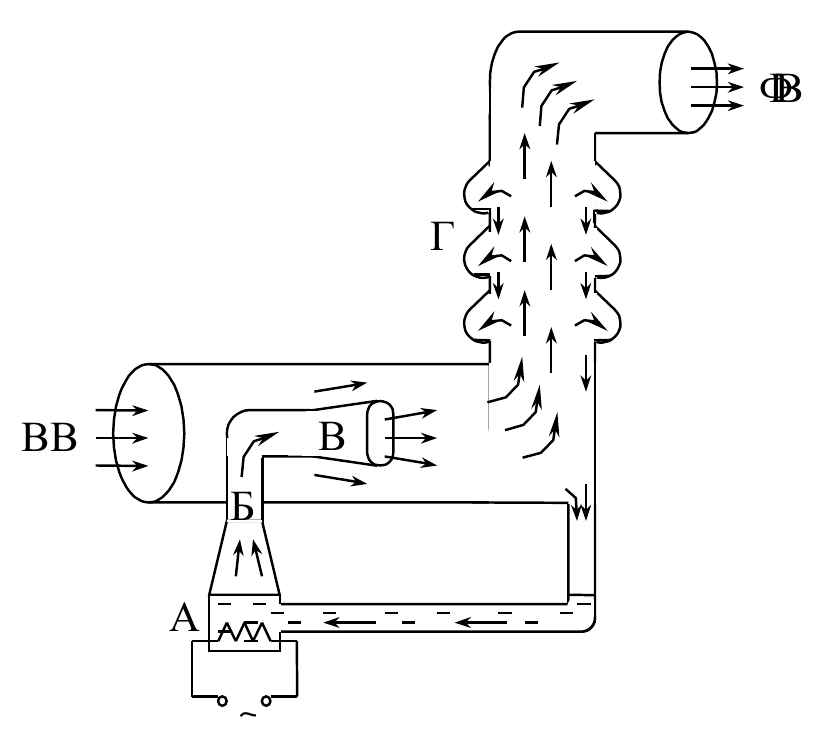
\includegraphics[width=0.5\textwidth]{diffuzionni_nasos.png}
        \caption{Схема одной ступени диффузионного насоса.}
        \label{ris:termoparni_monometr}
    \end{figure}
    \begin{figure}[h]
        \centering
        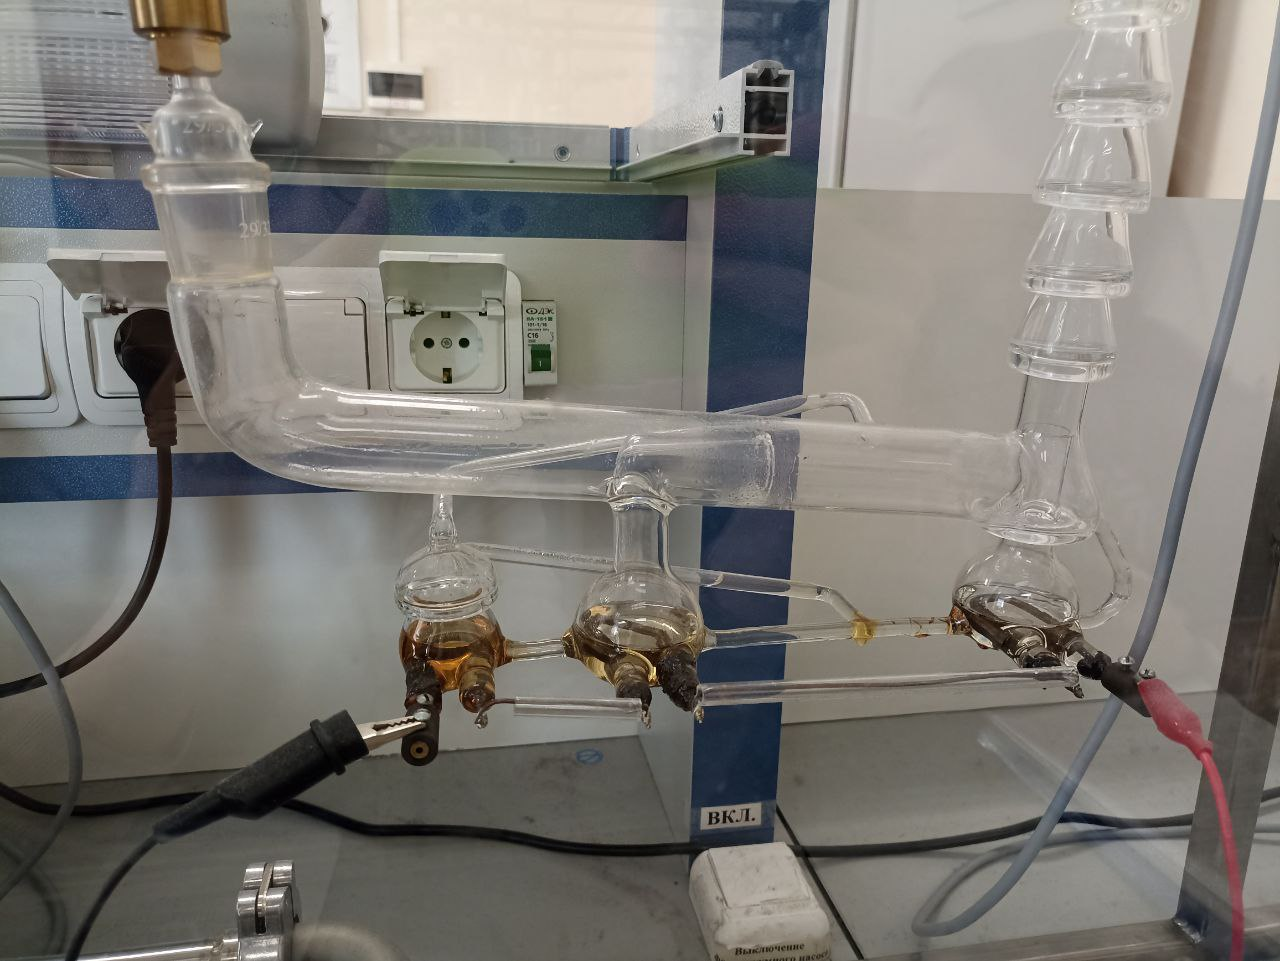
\includegraphics[width=0.6\textwidth]{photo_2025-05-06_01-23-33.jpg}
        \caption{Фото диффузионного насоса.}

    \end{figure}

    \section{Теоретическая часть}
    Производительность насоса определяется скоростью откачки $W$ (л/с): $W$ - это объем газа, удаляемого из сосуда при данном давлении за единицу времени. Скорость откачки форвакуумного насоса равна ёмкости воздухозаборной камеры, умноженной на число оборотов в секунду.\\
    Обозначим через $Q_\text{д}$ количество газа, десорбирующегося с поверхности откачиваемого объема в единицу времени, через $Q_\text{и}$ - количество газа, проникающего в единицу времени в этот объем извне - через течи, через $Q_\text{н}$ - поток газа, поступающего из насоса назад в откачивающую систему. Будем измерять их в единицах $PV$. Основное уравнение, описывающее процесс откачки, имеет вид
    \begin{equation*}
    	-VdP = (PW - Q_\text{д} - Q_\text{и} - Q_\text{н})dt.
    	\eqno(1)
    \end{equation*}
    При достижении предельного вакуума (давление $P_\text{пр}$)
    \begin{equation*}
    	\frac{dP}{dt} = 0,
    \end{equation*}
    так что
    \begin{equation*}
    	PW = Q_\text{д} + Q_\text{и} + Q_\text{н}.
    	\eqno(2)
    \end{equation*}
    Из этого уравнения получаем
    \begin{equation*}
    	W = \frac{\displaystyle \sum Q_i}{P_\text{пр}}.
    \end{equation*}
    Обычно $Q_\text{и}$ постоянно, а $Q_\text{д}$ и $Q_\text{н}$ слабо зависят от времени. Считая скорость откачки $W$ постоянной, уравнение (1) можно проинтегрировать и, используя (2), получить
    \begin{equation*}
    	P - P_\text{пр} = (P_0 - P_\text{пр}) e^{-\frac{t}{\tau}},
    	\eqno(3)
    \end{equation*}
    где $\tau = \frac{V}{W}$ является мерой эффективности откачки системы.\\
    Для количества газа, протекающего через трубу в условиях высокого вакуума справедлива формула
    \begin{equation*}
    	\frac{d(PV)}{dt} = \frac{4}{3} r^3 \sqrt{\frac{2\pi RT}{\mu}}\frac{P_2 - P_1}{L}.
    	\eqno(4)
    \end{equation*}
    Пренебрежем давлением $P_1$ у конца обращенного к насосу. Будем измерять количество газа, покидающего установку при давлении $P = P_2$. Пропускная способность трубы
    \begin{equation*}
    	C_\text{тр} = \left(\frac{dV}{dt}\right) = \frac{4}{3} \frac{r^3}{L} \sqrt{\frac{2\pi RT}{\mu}}.
    	\eqno(5)
    \end{equation*}
    Для пропускной способности отверстия имеем формулу 
    \begin{equation*}
    	C_\text{отв} = S\frac{\bar{v}}{4}.
    	\eqno(6)
    \end{equation*}

    \newpage
    \section{Приборы и данные}
    \begin{itemize}
        \item Вакуумметр Мерадат-ВИТ19ИТ2, тип первичного преобразователя ПМИ-2, погрешность в диапазоне $1\cdot10^{-4}$ Па до $5\cdot10^{-2}$ Па 35\% от измеряемой величины.
    	\item Вакуумметр Мерадат-ВИТ16Т4, тип первичного преобразователя ПМТ-2, погрешность в диапазоне $1\cdot10^{-3}$ торр до $0,2$ торр 30\% от измеряемой величины.
    	\item Источник питания GPR-711H30D, погрешность измерения $\pm(0,5 \% +2 ед.)$
    	\item Масляной манометр, погрешность измеряющей линейки 1 мм, плотность масла $\rho = 0,885 \ \frac{\text{г}}{\text{см}^3}$.
        \item Термогигрометр с функцией отображения давления testo 622, погрешность измерения давления 3 гПа, температуры - 0,4 $^\circ C$, влажности - 2\% в диапазоне от 0 до 90 \%
    \end{itemize}

    \section{Ход работы}
    \subsection{Оценка объема форвакуумной и высоковакуумной частей установки}

\begin{enumerate}
    \item Зафиксируем начальные параметры окружающей среды:
            \begin{equation*}
            	t = 22,2 ^\circ C,
            \end{equation*}
            \begin{equation*}
            	P_0 = 99,00 \text{ кПа},
            \end{equation*}
            \begin{equation*}
            	\varphi = 41,6 \%.
            \end{equation*}
    \item Через открытые краны К1 и К2 впускаем в систему атмосферный воздух.
    \item Перекрываем К5 и К6, запирая в объеме $V_{\text{зап}} = 50$ см$^3$ воздуха.
    \item После этого закрываем К1 и К2, включаем форвакуумный насос. Через К2 подключаем установку к насосу и откачиваем до давления  $1,8 \cdot 10^{-2}$ торр.
    \item Отключаем установку от насоса, повернув ручку К2, и вновь открываем К1.
    \item Закрываем К3, изолируя высоковакуумную (ВВ) часть от форвакуумной (ФВ).
    \item Перекрываем кран К4.
    \item Открываем К5 и считываем уровни масла с обеих сторон манометра, чтобы определить давление $P_1$. Результаты заносим в таблицу.
    
    \begin{table}[H]
        \centering
        \begin{tabular}{|c|c|c|c|}
            \hline
            $h_1$, см & $h_2$, см  & $h_3$, см & $h_4$, см  \\\hline
            $11,6 \pm 0,1$ & $37,9 \pm 0,1$ &  $16,4 \pm 0,1$ & $33,3 \pm 0,1$  \\\hline
        \end{tabular}
        \caption{Результаты измерений уровней масла и давления}
    \end{table}

   \item
Теперь рассчитаем объем форвакуумной $V_\text{фв}$ и высоковакуумной $V_\text{вв}$ частей с помощью закона Бойля-Мариотта.

     $\Delta h' = h_2 - h_1 = 26,3 \pm 0,2\text{ см}$ \ \ $\Delta h'' = h_4 - h_3 = 16,9 \pm 0,2\text{ см}$.

    \begin{equation*}
    	V_\text{фв} = V_{\text{зап}} \left( \frac{P_0}{\rho_{\text{масло}} g \Delta h'} - 1 \right) = 0{,}05 \cdot \left( \frac{99000}{885 \cdot 9{,}81 \cdot 0{,}263} - 1 \right) \approx 2{,}118 \text{ л},
    \end{equation*}
    \begin{equation*}
    	V_\text{вв} = V_{\text{зап}} \left( \frac{P_0}{\rho_{\text{масло}} g \Delta h''} - 1 \right) - V_\text{фв} = 0{,}05 \cdot \left( \frac{99000}{885 \cdot 9{,}81 \cdot 0{,}169} - 1 \right) - 2{,}118 \approx  1{,}206 \text{ л},
    \end{equation*}
    \begin{equation*}
    \sigma_{V_\text{фв}} = \left(V_\text{фв} + V_{\text{зап}}\right) \cdot \sqrt{ \left( \frac{V_\text{фв}}{V_\text{фв} + V_{\text{зап}}} \frac{\sigma_{V_{\text{зап}}}}{V_{\text{зап}}} \right)^2 + \left( \frac{\sigma_\rho}{\rho} \right)^2 + \left( \frac{\sigma_h}{h} \right)^2 + \left( \frac{\sigma_P}{P} \right)^2 } =
    \end{equation*}
    \begin{equation*}
    = \sqrt{ \left( 0{,}004 \right)^2 + \left( 0{,}002 \right)^2 + \left( 0{,}017 \right)^2 + \left( 0{,}007 \right)^2 } = 0{,}018 \text{ л},
    \end{equation*}
    \begin{equation*}
    \sigma_{V_\text{вв}}  = 0{,}060 \text{ л},
    \end{equation*}
    
    \item В итоге получаем вот такие объёмы: $V_\text{фв} = 2{,}118 \pm 0{,}018$ ($\varepsilon_\text{фв} = 0{,}87\,\%$), $V_\text{вв} = 1{,}206 \pm 0{,}060$ ($\varepsilon_\text{вв} = 5{,}00\,\%$)
    
    
    \end{enumerate}

\subsection{Достижение высокого вакуума и определение скорости откачки}

\begin{enumerate}
    \setcounter{enumi}{10}
    \item Открываем все краны и производим предварительную откачку системы до давления порядка $1 \cdot 10^{-2}$ торр.

    \item Подаём ток $I = 0{,}6$ А на диффузионный насос и ждём около 5 минут для прогрева масла. Затем плавно увеличиваем ток до $1{,}27$ А.
    
    \item После достижения давления порядка $3 \cdot 10^{-4}$ торр включаем ионизационный манометр.
    
    \item При снижении давления до $1 \cdot 10^{-4}$ торр начинаем дегазацию.
    
    \item После установленного времени дегазации достигаем предельного давления:
    \[
        P_{\text{пр}} = (8{,}30 \pm 2{,}91) \cdot 10^{-5} \text{ торр}.
    \]
    
    \item Закрываем кран $K_3$, отключая откачку высоковакуумной части, и с помощью видеокамеры фиксируем рост давления до $\sim 5 \cdot 10^{-4}$ торр.
    
    \item Затем вновь открываем $K_3$ и наблюдаем восстановление вакуума. Повторяем этот цикл дважды.
    
    \item По полученным данным строим зависимость давления от времени $P(t)$.
    
    \item Для участка восстановления вакуума (экспоненциальный спад) строим график зависимости $\ln(P - P_{\text{пр}})$. Все графики представлены в приложении работы.

    \item В результате аппроксимации линейных участков графиков зависимости давления от времени были получены следующие значения скоростей изменения давления:
    
    \[
        k_1^{\text{lin}} = (1{,}312 \pm 0{,}005) \cdot 10^{-5} \ \frac{\text{торр}}{\text{с}}, \qquad
        k_2^{\text{lin}} = (1{,}323 \pm 0{,}006) \cdot 10^{-5} \ \frac{\text{торр}}{\text{с}}.
    \]
    
    Для экспоненциальных участков восстановления вакуума рассчитаны соответствующие постоянные времени:
    
    \[
        \tau_1 = \frac{1}{k_1^{\text{exp}}} = (5{,}84 \pm 0{,}16) \ \text{с}, \qquad
        \tau_2 = \frac{1}{k_2^{\text{exp}}} = (5{,}85 \pm 0{,}17) \ \text{с}.
    \]
    
    Среднее значение постоянной времени, учитывающее оба эксперимента, составляет:
    
    \[
        \tau = \frac{\tau_1 + \tau_2}{2} = (5{,}85 \pm 0{,}17) \ \text{с}.
    \]
    
    \item Зная объём исследуемой области установки $V_{\text{вв}} = 1{,}206$ л, рассчитаем эффективную скорость откачки:
    
    \[
        W = \frac{V_{\text{вв}}}{\tau} = \frac{1{,}206}{5{,}85} = 0{,}206 \ \frac{\text{л}}{\text{с}}.
    \]
    
    Погрешность определения $W$:
    
    \[
        \sigma_W =  W \sqrt{\left(\frac{\sigma_{V_\text{вв}}}{V_\text{вв}}\right)^2 +\left(\frac{\sigma_{\tau}}{\tau}\right)^2} = 0{,}206 \cdot \sqrt{\left( 0{,}05\right)^2 + \left(0{,}03\right)^2} = 0{,}012 \ \frac{\text{л}}{\text{с}}.
    \]
    
    Относительная погрешность:
    
    \[
        \varepsilon_W =  5{,}83\%.
    \]
    
    \item Для оценки потока газа $Q_{\text{н}}$, возвращающегося из насоса в систему, используем выражение:
    
    \[
        V_{\text{вв}} \frac{dP}{dt} = Q_\text{д} + Q_\text{и}.
    \]
    
    В качестве средней скорости изменения давления используем:
    
    \[
        \bar{k} = \frac{k_1^{\text{lin}} + k_2^{\text{lin}}}{2} = (1{,}318 \pm 0{,}006) \cdot 10^{-5} \ \frac{\text{торр}}{\text{с}}.
    \]
    
    С учётом уравнения баланса потоков $PW = Q_\text{д} + Q_\text{и} + Q_\text{н}$, выражаем:
    
    \[
        Q_\text{н} = P_{\text{пр}} W - \bar{k} V_{\text{вв}} = 8{,}30 \cdot 10^{-5} \cdot 0{,}206 - 1{,}319 \cdot 10^{-5} \cdot 1{,}206 = 1{,}2 \cdot 10^{-6} \ \frac{\text{торр} \cdot \text{л}}{\text{с}}.
    \]
    
    Расчёт полной погрешности:
    
    \[
        \sigma_{Q_\text{н}} = \sqrt{(\sigma_{P_{\text{пр}}} W)^2 + (P_{\text{пр}} \sigma_W)^2} + \sqrt{(\sigma_{V_{\text{вв}}} \bar{k})^2 + (V_{\text{вв}} \sigma_{\bar{k}})^2} = 7,6 \cdot 10^{-6} \ \frac{\text{торр} \cdot \text{л}}{\text{с}}
    \]
    
    Таким образом, метод позволяет лишь приблизительно оценить порядок величины $Q_{\text{н}}$.


    
   \end{enumerate}

   \subsection{Метод введения искусственной течи}

    В ходе эксперимента была создана искусственная течь с помощью открытия крана $K_5$. Через 3--5 минут были зафиксированы установившиеся давления:
    
    \begin{itemize}
        \item Давление в системе: $P_{\text{уст}} = (1{,}60 \pm 0{,}56) \cdot 10^{-4} \ \text{торр}$
        \item Давление со стороны форвакуумной части: $P_{\text{фв}} = (5{,}40 \pm 1{,}62) \cdot 10^{-3} \ \text{торр}$
        \item Остаточное предельное давление: $P_{\text{пр}} = (8{,}3 \pm 1{,}0) \cdot 10^{-5} \ \text{торр}$
    \end{itemize}
    
    Размеры капилляра, используемого в системе:
    \[
    r = (0{,}80 \pm 0{,}10) \ \text{мм}, \quad L = (10{,}8 \pm 0{,}1) \ \text{см}
    \]
    
    Расчитаем по данным формулам:
    
    \begin{align*}
    C_{\text{кап}} &= \frac{4}{3} \frac{(r)^3}{L} \sqrt{\frac{2\pi R T}{\mu}} = 5{,}76 \cdot 10^{-7} \ \frac{\text{м}^3}{\text{с}} \\
    \sigma_{C_{\text{кап}}} &= C_{\text{кап}} \cdot \sqrt{\left( \frac{3\sigma_r}{r} \right)^2 + \left( \frac{\sigma_L}{L} \right)^2 + \left( \frac{\sigma_T}{T} \right)^2} = 2{,}16 \cdot 10^{-7} \ \frac{\text{м}^3}{\text{с}}
    \end{align*}
    
    Расчёт производительности вакуумной системы:
    
    \[
    W = \frac{C_{\text{кап}}(P_{\text{фв}} - P_{\text{уст}})}{P_{\text{уст}} - P_{\text{пр}}} = 0{,}04 \ \frac{\text{л}}{\text{с}}
    \]
    
    Оценка погрешности:
    
    \begin{align*}
    \sigma_W &= C_{\text{кап}} \cdot \sqrt{
    \left( \frac{\partial W}{\partial P_{\text{фв}}} \cdot \frac{\sigma_{P_{\text{фв}}}}{C_{\text{кап}}} \right)^2 +
    \left( \frac{\partial W}{\partial P_{\text{уст}}} \cdot \frac{\sigma_{P_{\text{уст}}}}{C_{\text{кап}}} \right)^2 +
    \left( \frac{\partial W}{\partial P_{\text{пр}}} \cdot \frac{\sigma_{P_{\text{пр}}}}{C_{\text{кап}}} \right)^2 +
    \left( \frac{\partial W}{\partial C_{\text{кап}}} \cdot \frac{\sigma_{C_{\text{кап}}}}{C_{\text{кап}}} \right)^2 } \\
    &= 3{,}77 \cdot 10^{-5} \ \frac{\text{м}^3}{\text{с}}, \quad \varepsilon_W = 96\%
    \end{align*}
    
    \textbf{Вывод:} полученное значение производительности $W \approx 0{,}04 \ \frac{\text{л}}{\text{с}}$ сопровождается большой относительной погрешностью, что свидетельствует о низкой точности метода искусственной течи.

    \section{Обсуждения и результаты}
    
    \begin{itemize}
    
    \item Объёмы форвакуумного и высоковакуумного резервуаров были определены с хорошей точностью:

    $V_\text{фв} = 2{,}118 \pm 0{,}018 \ \text{л} \quad (\varepsilon_\text{фв} = 0{,}87\%), \quad V_\text{вв} = 1{,}206 \pm 0{,}060 \ \text{л} \quad (\varepsilon_\text{вв} = 5{,}00\%)$

    
    \item На графиках наблюдается линейный рост давления при поступлении воздуха и экспоненциальное уменьшение давления при откачке. \\[0.5ex]
    На основании графиков 3 и 4 получено значение характерного времени откачки: \\[0.5ex]
    \begin{math}
        \tau = (5{,}85 \pm 0{,}17) \ \text{с}
    \end{math}
    
    \item Скорость откачки $W$ была рассчитана двумя методами: \\[0.5ex]
    первый — по улучшению вакуума, второй — по созданной искусственной течи. Результаты сведены в таблицу ниже:
    
    \begin{table}[H]
        \centering
        \begin{tabular}{|c|c|c|c|}
            \hline
            Метод & $W,\ \frac{\text{л}}{\text{с}}$ & $\sigma_W,\ \frac{\text{л}}{\text{с}}$ & $\varepsilon_W,\ \%$ \\
            \hline
            1 & $0{,}206$ & $0{,}012$ & $5{,}8$ \\
            \hline
            2 & $0{,}039$ & $0{,}038$ & $96{,}1$ \\
            \hline
        \end{tabular}
        \caption{Результаты определения скорости откачки двумя методами}
\end{table}

Метод 1 оказался достаточно надёжным: относительная погрешность составляет около 6~\%. Метод 2 демонстрирует высокую неопределённость (погрешность почти равна самой величине), что связано с сильным влиянием ошибок измерения радиуса трубки, от которого результат зависит в кубе. Его можно использовать лишь для приближённой оценки.

\item Оценка обратного потока газа из насоса дала значение: \\[0.5ex]
\begin{math}
    Q_\text{н} = (1{,}2 \pm 7{,}6) \cdot 10^{-6} \ \frac{\text{торр} \cdot \text{л}}{\text{с}}
\end{math} \\[0.5ex]
При этом большая величина погрешности указывает на ориентировочный характер результата.

\end{itemize}

    \section{Выводы}
Были вычислены с помощью вакуумной установки, манометров и закона Бойля-Мариотта объемы форвакуумного и высоковакуумного баллонов. С помощью двух методов определили скорость откачки насоса. Построили графики зависимостей $P(t)$ и $\ln(P - P_\text{пр})$. Оценили значение для потока газа, поступающего из насоса назад в откачиваемую систему.


    \section{Приложение}

    
    \begin{figure}[!h]
        \center{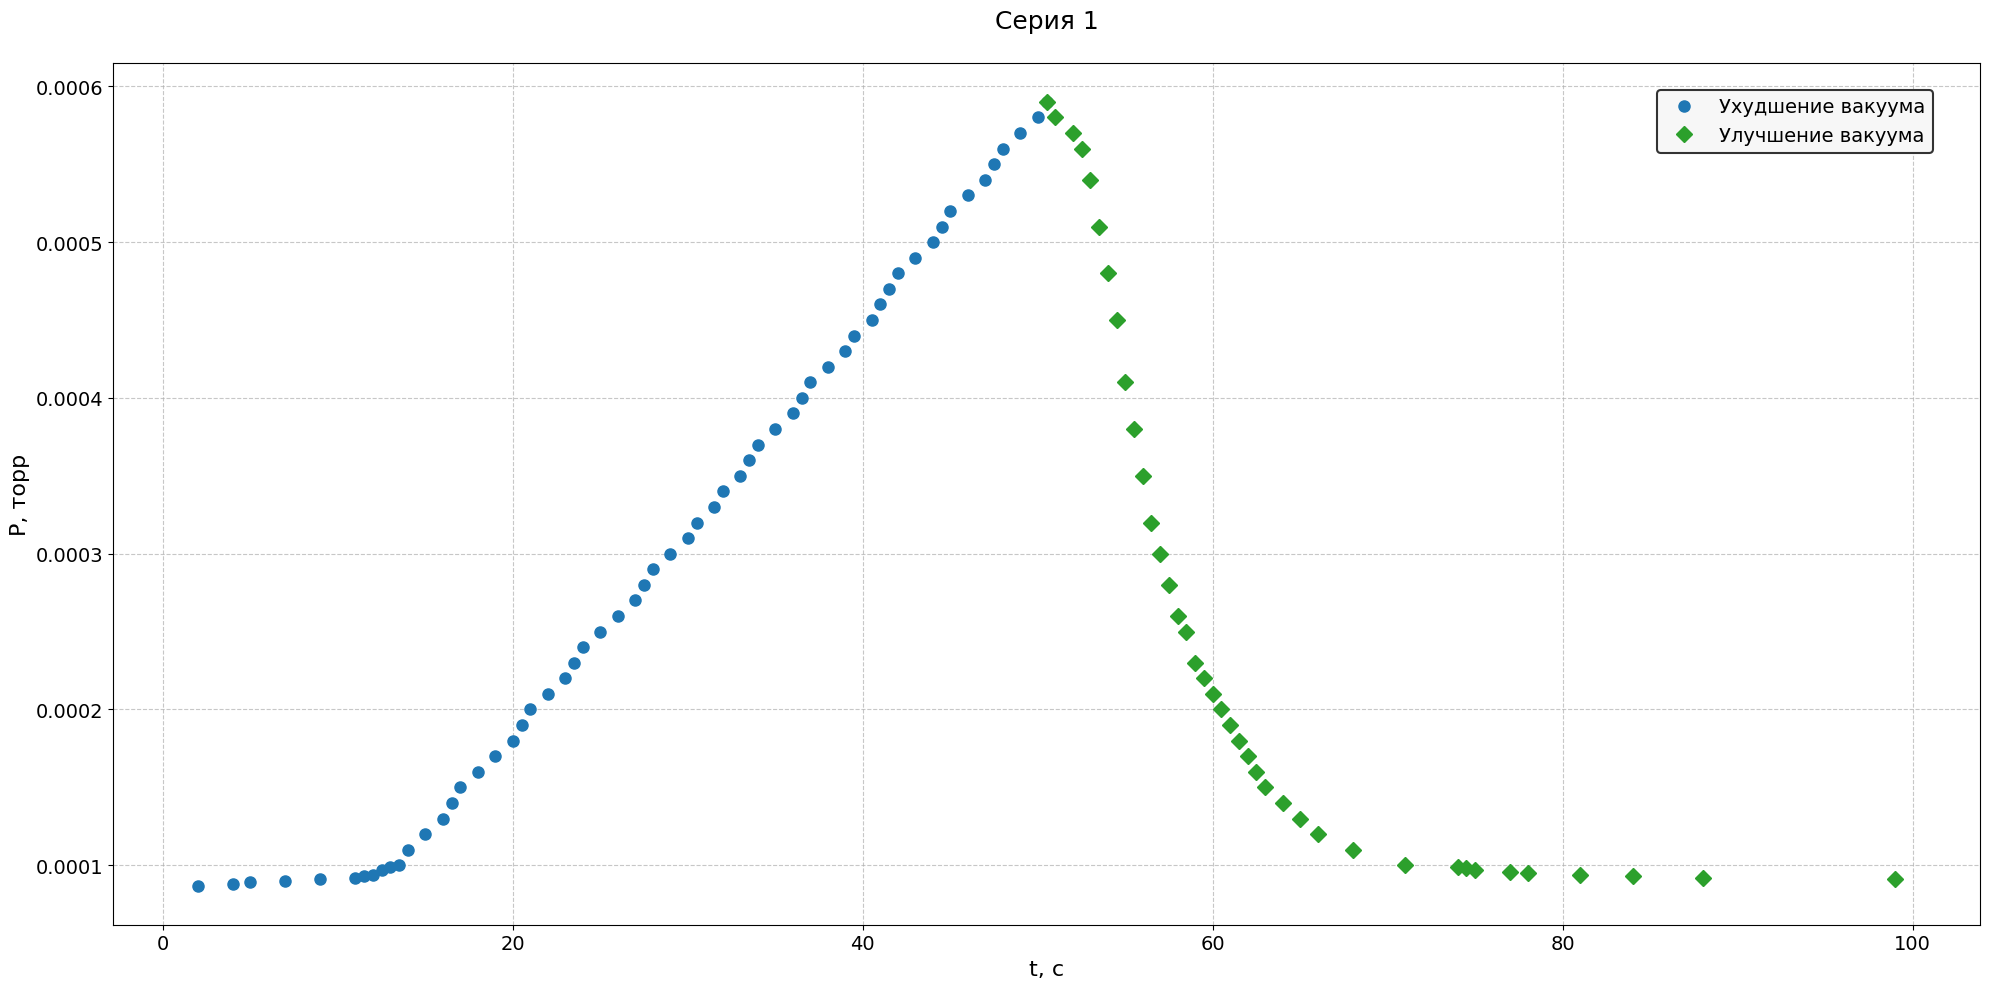
\includegraphics[width=1\textwidth]{graphs/ser1.png}}
        \caption{Первая серия опыта}
    \end{figure}
    \begin{figure}[!h]
        \center{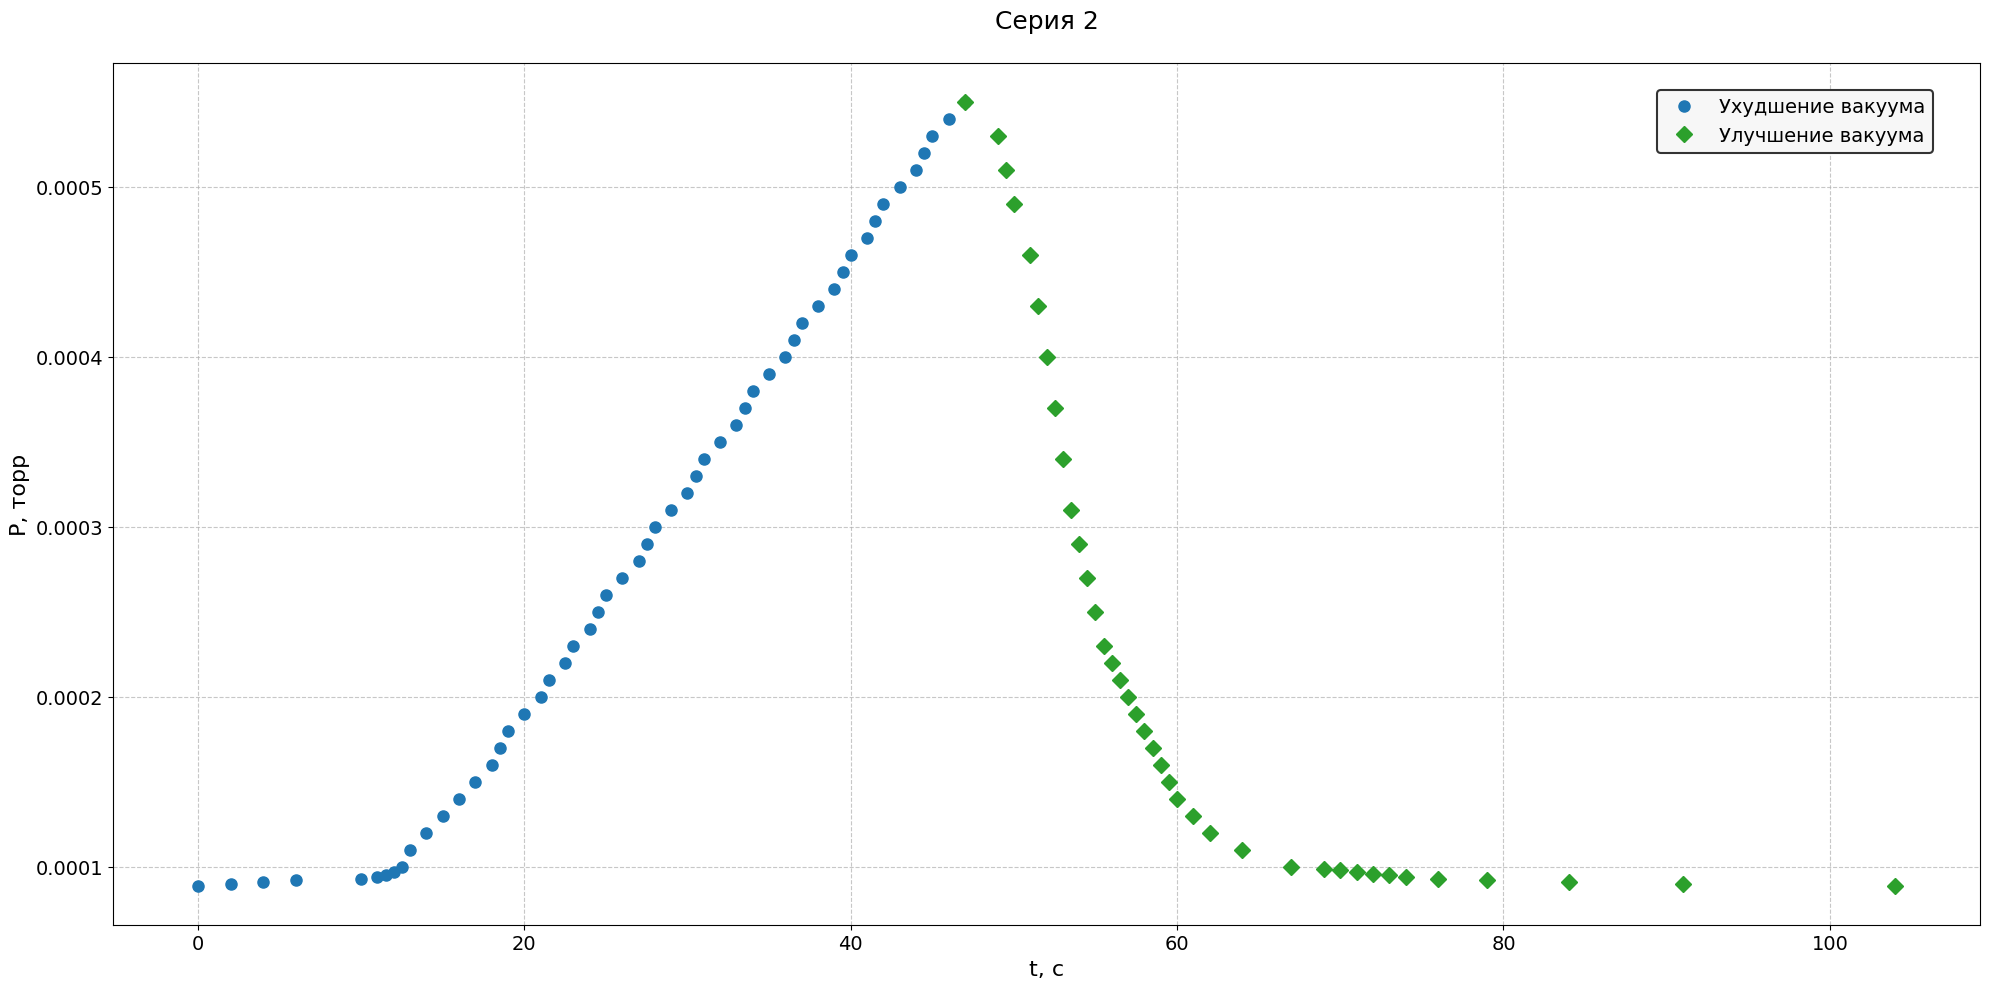
\includegraphics[width=1\textwidth]{graphs/ser2.png}}
        \caption{Вторая серия опыта}
    \end{figure}

    \begin{figure}[!h]
        \center{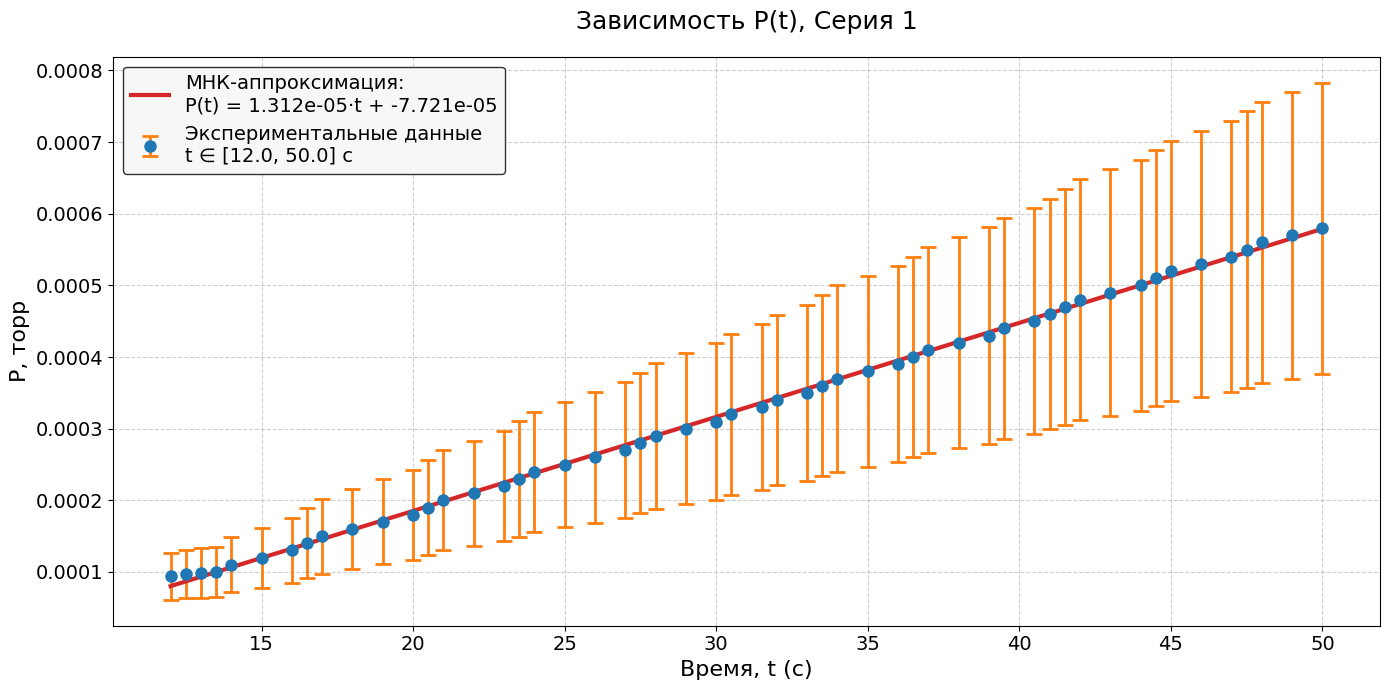
\includegraphics[width=1\textwidth]{graphs/uhu1.png}}
        \caption{Ухудшение вакуума}
    \end{figure}
    \begin{figure}[!h]
        \center{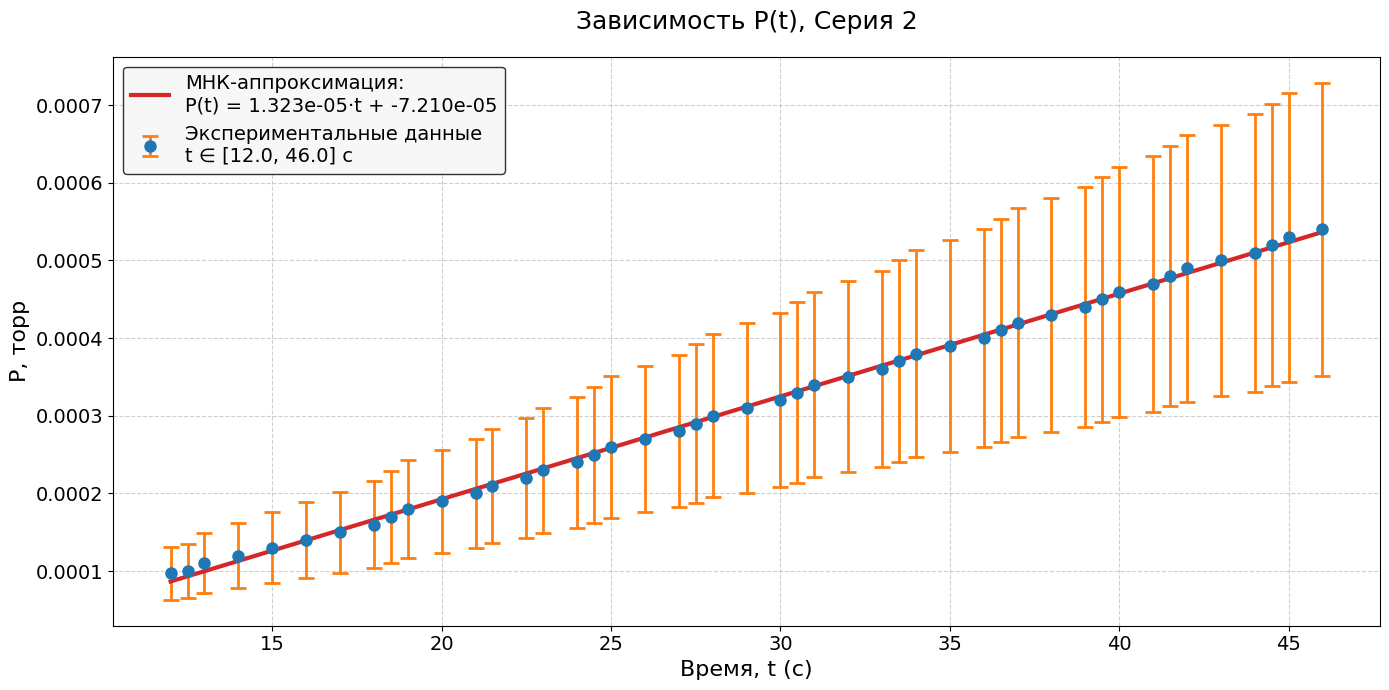
\includegraphics[width=1\textwidth]{graphs/uhu2.png}}
        \caption{Ухудшение вакуума}
    \end{figure}

    \begin{figure}[!h]
        \center{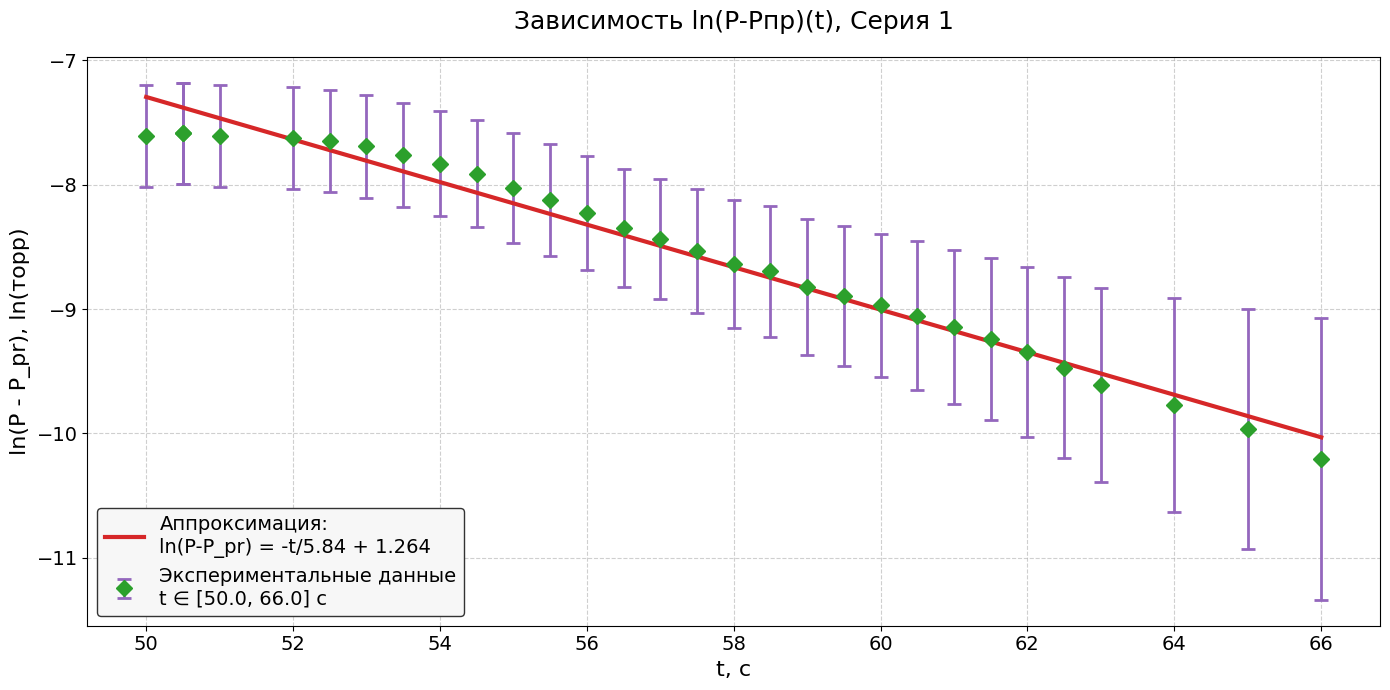
\includegraphics[width=1\textwidth]{graphs/ulu1.png}}
        \caption{Улучшение вакуума}
    \end{figure}
    \begin{figure}[!h]
        \center{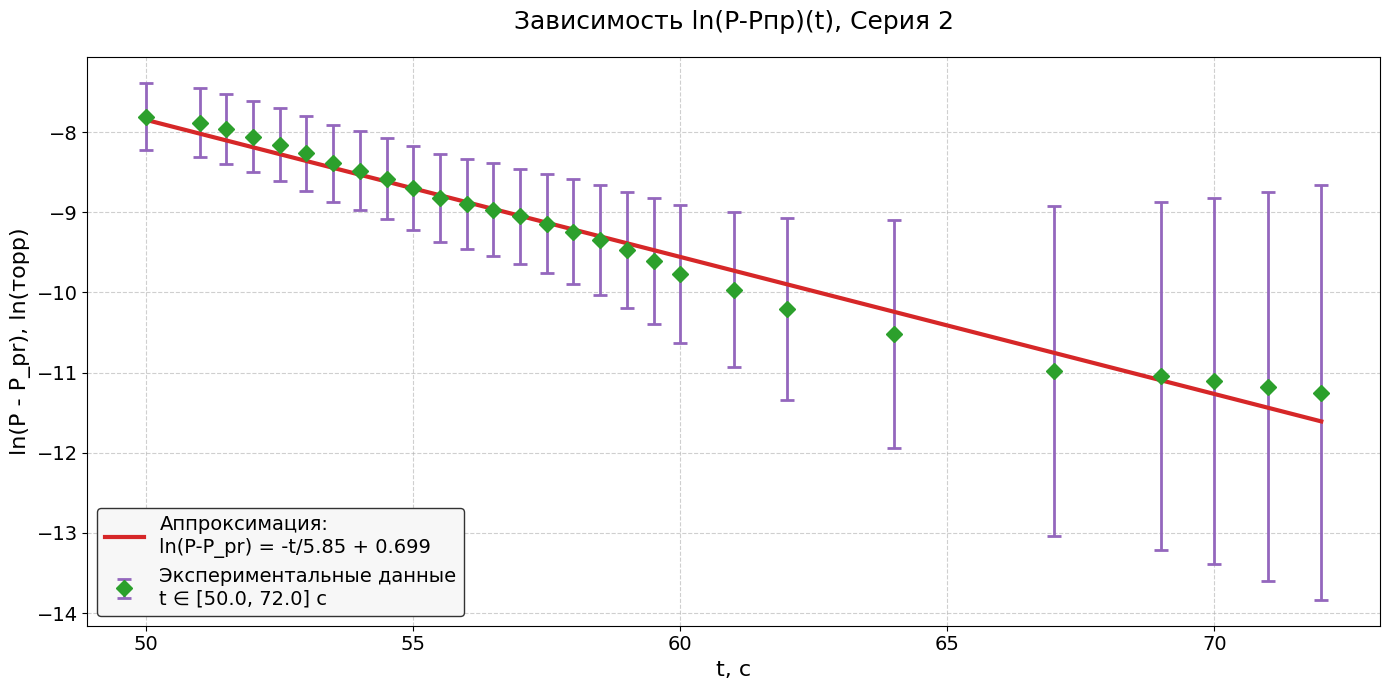
\includegraphics[width=1\textwidth]{graphs/ulu2.png}}
        \caption{Улучшение вакуума}
    \end{figure}

\end{document}
